\documentclass[tikz,border=6pt]{standalone}
\usepackage{pgfplots}
\usepackage{amsmath}
\usetikzlibrary{
  arrows.meta,
  backgrounds,
  calc,
  fit,
  matrix,
  positioning,
  shapes.callouts,
  shapes.geometric,
  shapes.misc
}
\pgfplotsset{compat=1.18}

\definecolor{archInk}{HTML}{1F2933}
\definecolor{archBlue}{HTML}{0B4F6C}
\definecolor{archTeal}{HTML}{1B998B}
\definecolor{archGold}{HTML}{D98E04}
\definecolor{archRose}{HTML}{C44536}
\definecolor{archSage}{HTML}{7A9E7E}
\definecolor{archMist}{HTML}{E9F1F7}
\definecolor{archSand}{HTML}{F4F1DE}
\definecolor{archSlate}{HTML}{5C677D}
\definecolor{archStone}{HTML}{C8D0D9}

\tikzset{
  every node/.style={font=\sffamily\small, text=archInk},
  axis label/.style={font=\sffamily\footnotesize, text=archInk},
  panel/.style={
    rounded corners=6pt,
    draw=archSlate,
    line width=0.9pt,
    fill=white
  },
  stage/.style={
    panel,
    fill=archMist,
    minimum height=1.5cm,
    inner sep=7pt,
    align=left
  },
  note/.style={
    panel,
    fill=archSand,
    inner sep=7pt,
    align=left
  },
  verdict/.style={
    panel,
    fill=archTeal!12,
    inner sep=7pt,
    align=left
  },
  kill/.style={
    panel,
    fill=archRose!12,
    draw=archRose,
    inner sep=7pt,
    align=left
  },
  muted/.style={
    panel,
    fill=archStone!20,
    draw=archStone!80!archInk,
    inner sep=6pt,
    align=left
  },
  link/.style={
    -{Latex[length=3mm,width=1.7mm]},
    line width=1.0pt,
    draw=archBlue
  },
  dashedlink/.style={
    -{Latex[length=3mm,width=1.7mm]},
    line width=1.0pt,
    draw=archRose,
    dashed
  }
}

\pgfplotsset{
  every axis/.append style={
    line width=0.9pt,
    tick style={draw=archSlate},
    axis line style={draw=archSlate},
    label style={font=\sffamily\small, text=archInk},
    ticklabel style={font=\sffamily\footnotesize, text=archInk},
    legend style={
      draw=none,
      fill=white,
      font=\sffamily\footnotesize,
      text=archInk
    },
    title style={font=\sffamily\small\bfseries, text=archInk},
    grid style={draw=archStone},
    major grid style={draw=archStone},
    minor grid style={draw=archStone!70}
  }
}

\begin{document}
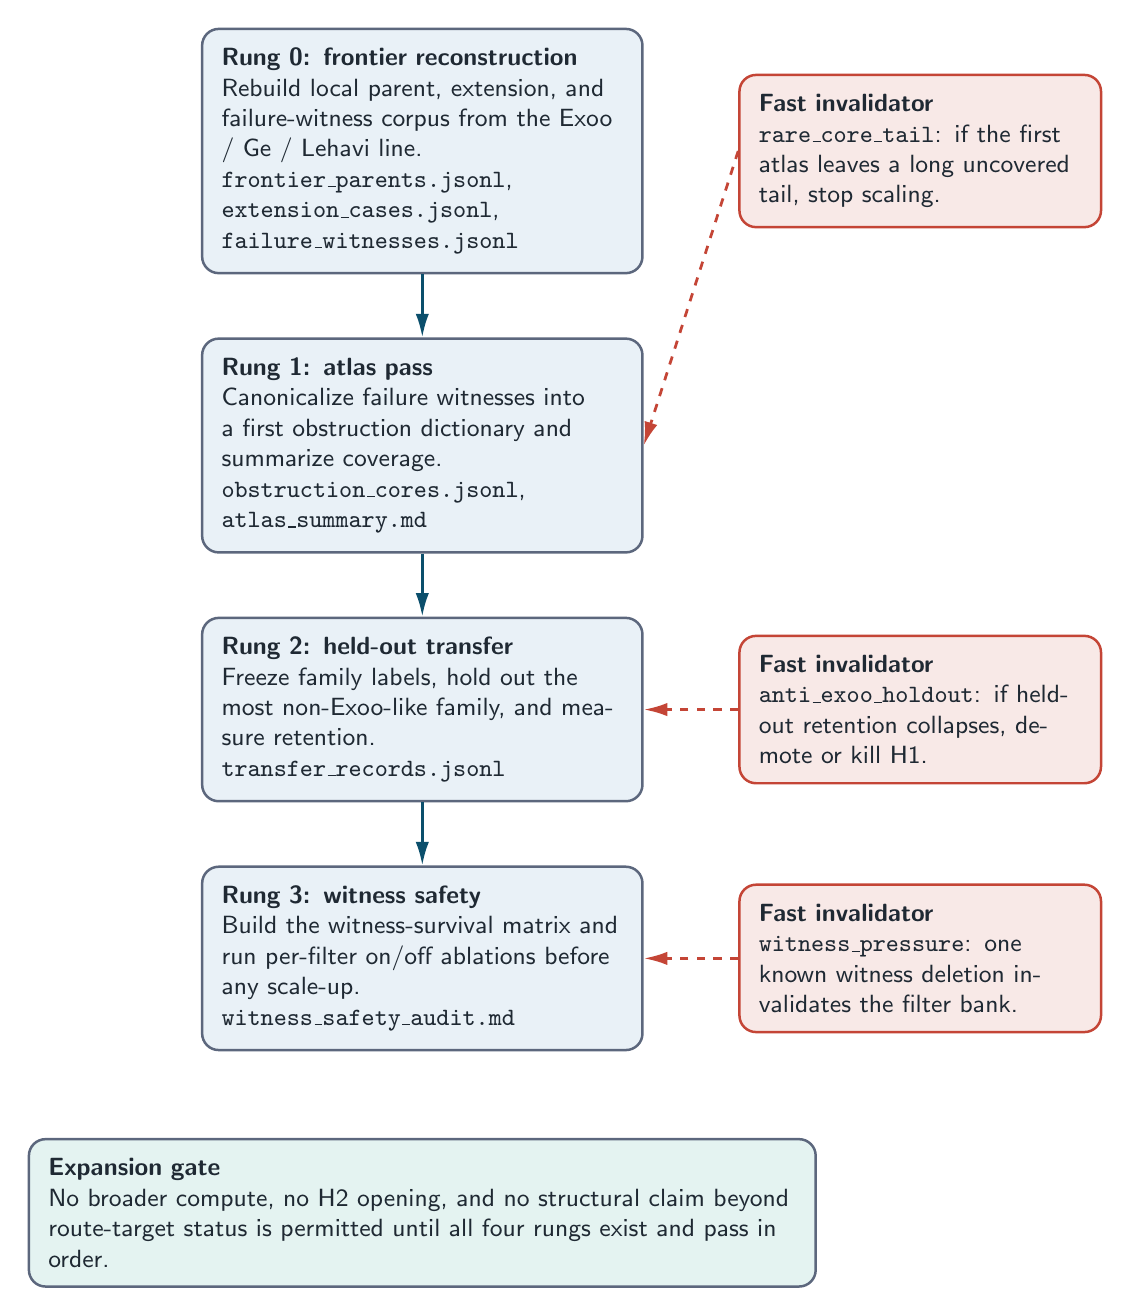
\begin{tikzpicture}[node distance=8mm and 12mm]
  \node[stage, text width=5.1cm] (r0) {
    \textbf{Rung 0: frontier reconstruction}\\
    Rebuild local parent, extension, and failure-witness corpus from the Exoo / Ge / Lehavi line.\\
    \texttt{frontier\_parents.jsonl}, \texttt{extension\_cases.jsonl}, \texttt{failure\_witnesses.jsonl}
  };
  \node[stage, text width=5.1cm, below=of r0] (r1) {
    \textbf{Rung 1: atlas pass}\\
    Canonicalize failure witnesses into a first obstruction dictionary and summarize coverage.\\
    \texttt{obstruction\_cores.jsonl}, \texttt{atlas\_summary.md}
  };
  \node[stage, text width=5.1cm, below=of r1] (r2) {
    \textbf{Rung 2: held-out transfer}\\
    Freeze family labels, hold out the most non-Exoo-like family, and measure retention.\\
    \texttt{transfer\_records.jsonl}
  };
  \node[stage, text width=5.1cm, below=of r2] (r3) {
    \textbf{Rung 3: witness safety}\\
    Build the witness-survival matrix and run per-filter on/off ablations before any scale-up.\\
    \texttt{witness\_safety\_audit.md}
  };

  \draw[link] (r0) -- (r1);
  \draw[link] (r1) -- (r2);
  \draw[link] (r2) -- (r3);

  \node[kill, text width=4.1cm, right=of r0] (k0) {
    \textbf{Fast invalidator}\\
    \texttt{rare\_core\_tail}: if the first atlas leaves a long uncovered tail, stop scaling.
  };
  \node[kill, text width=4.1cm, right=of r2] (k1) {
    \textbf{Fast invalidator}\\
    \texttt{anti\_exoo\_holdout}: if held-out retention collapses, demote or kill H1.
  };
  \node[kill, text width=4.1cm, right=of r3] (k2) {
    \textbf{Fast invalidator}\\
    \texttt{witness\_pressure}: one known witness deletion invalidates the filter bank.
  };

  \draw[dashedlink] (k0.west) -- (r1.east);
  \draw[dashedlink] (k1.west) -- (r2.east);
  \draw[dashedlink] (k2.west) -- (r3.east);

  \node[verdict, text width=9.5cm, below=11mm of r3] (gate) {
    \textbf{Expansion gate}\\
    No broader compute, no H2 opening, and no structural claim beyond route-target status is
    permitted until all four rungs exist and pass in order.
  };
\end{tikzpicture}
\end{document}
